\documentclass[a4paper, 12pt]{article}
\usepackage{geometry}
\geometry{verbose,a4paper,tmargin=2cm,bmargin=2cm,lmargin=2cm,rmargin=2cm}
\usepackage{fontspec}
\setmainfont[
  Ligatures=TeX,
  Extension=.otf,
  UprightFont=*-regular,
  ItalicFont=*-italic,
  BoldFont=*-bold,
  BoldItalicFont=*-bolditalic,
]{xits}
\usepackage[english,russian]{babel}

\newif\ifisinsp
\newif\ifisone
\newif\ifisname
\newif\ifisnum
\isinsptrue
\isonetrue
\isnamefalse
\isnumtrue

\def \labtype {Лабораторная}
% Это для нумерации страниц после титульника
\usepackage{fancyhdr}
\pagestyle{fancy}
\renewcommand{\headrulewidth}{0pt}
\fancyfoot[C] {\thepage}

\isonefalse
\def \labnum {2}
\def \labsubj {Тестирование программного обеспечения}
\def \labauthor {Айтуганов Д. А. \\ Чебыкин И. Б.}
\def \labgroup {P3301}
\isinspfalse
\def \labinsp {}
\def \labname {Вариант: 633}
\isnametrue

\usepackage{graphicx}
\usepackage{verbatim}
\usepackage[dvipsnames]{xcolor}

\usepackage{fancyvrb}

\RecustomVerbatimCommand{\VerbatimInput}{VerbatimInput} {
 fontsize=\scriptsize,
 %
 frame=lines,  % top and bottom rule only
 framesep=2em, % separation between frame and text
 rulecolor=\color{Gray},
 %
 label=\fbox{\color{Black}source},
 labelposition=topline,
 %
}

\begin{document}
\begin{titlepage}
	\begin{center}
		\large
		Университет ИТМО

		\vspace{0.25cm}
		
		Факультет программной инженерии и компьютерной техники
		
		Кафедра вычислительной техники
		\vfill
		
		\textsc{\labtype\spaceработа \ifisnum № \labnum{} \fi по дисциплине \\"\labsubj" \ifisname\small \\ \labname \fi}
			
		\bigskip
	\end{center}
	\vfill
	\vfill
	
	\begin{flushright}
	\ifisone
	Выполнил: \labauthor
	\else
	Выполнили: \labauthor
	\fi

	\vspace{0.25cm}
	Группа: \labgroup
			
	\vspace{0.25cm}
	\ifisinsp
	Проверяющий: \labinsp
	\fi
	\end{flushright}
	\vfill
	
	\begin{center}
	СПб, \the\year
	\end{center}
\end{titlepage}

\section{Задание}

Провести интеграционное тестирование программы, осуществляющей вычисление
системы функций.
\begin{enumerate}
\item Все составляющие систему функции (как тригонометрические,
так и логарифмические) должны быть выражены через базовые (тригонометрическая
зависит от варианта; логарифмическая - натуральный логарифм).
\item Структура приложения, тестируемого в рамках лабораторной работы, должна
выглядеть следующим образом (пример приведён для базовой тригонометрической
функции sin(x)):
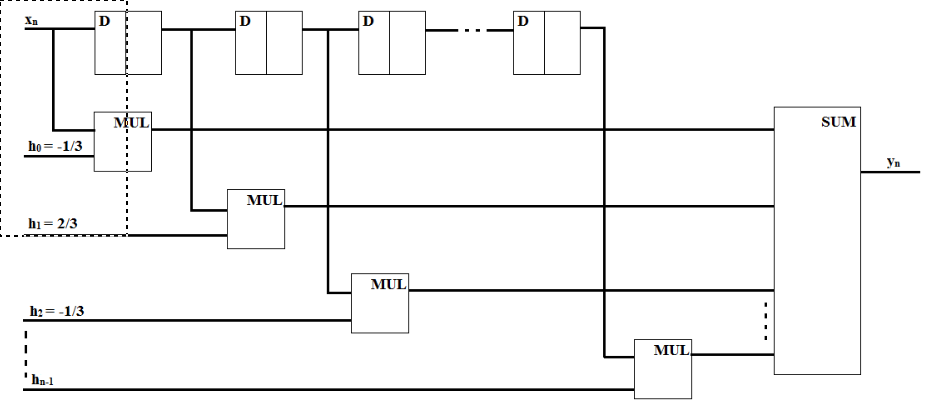
\includegraphics[width=400bp]{img/scheme.png}

\item Обе "базовые" функции (в примере выше - sin(x) и ln(x)) должны быть
реализованы при помощи разложения в ряд с задаваемой погрешностью.
Использовать тригонометрические / логарифмические преобразования
для упрощения функций ЗАПРЕЩЕНО. Для КАЖДОГО модуля должны быть реализованы
табличные заглушки. При этом, необходимо найти область допустимых
значений функций, и, при необходимости, определить взаимозависимые точки в модулях.
\item Разработанное приложение должно позволять выводить значения, выдаваемое
любым модулем системы, в сsv файл вида «X, Результаты модуля (X)», позволяющее
произвольно менять шаг наращивания Х. Разделитель в файле csv можно использовать
произвольный.
\end{enumerate}

Порядок выполнения работы:

\begin{enumerate}
\item Разработать приложение, руководствуясь приведёнными выше правилами.
\item С помощью JUNIT4 разработать тестовое покрытие системы функций,
проведя анализ эквивалентности и учитывая особенности системы функций.
Для анализа особенностей системы функций и составляющих ее частей можно
использовать сайт \\ https://www.wolframalpha.com/.
\item Собрать приложение, состоящее из заглушек.  Провести интеграцию приложения
по 1 модулю, с обоснованием стратегии интеграции, проведением интеграционных
тестов и контролем тестового покрытия системы функций.
\end{enumerate}
\subsection{Система уравнений}
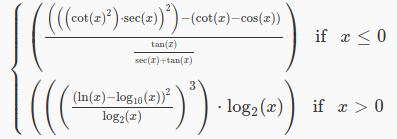
\includegraphics[width=300bp]{img/system.png}
\section{Выполнение}
\subsection{Диаграмма классов}
\includegraphics[width=400bp]{img/uml.png}
\subsection{Описание тестового покрытия}
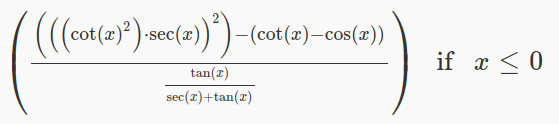
\includegraphics[width=300bp]{img/first.png}

Функция периодичная, определена на $-\frac{\pi}{2} < x - 2\pi m < 0$

Краевые точки:

$\pi < x < 0$

$x = -1,5708, y = 0$

$x = -2,1904, y = 0.1202$

$x = -2,3197, y = 0$

$2\pi < x < \pi$

$x = -4,713, y = 0$

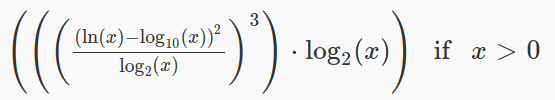
\includegraphics[width=300bp]{img/second.png}

$0 < x < 1$

$x = 0, y = NaN$

$x = 1, y = NaN$

$1 < x < \infty$
\subsection{Графики}


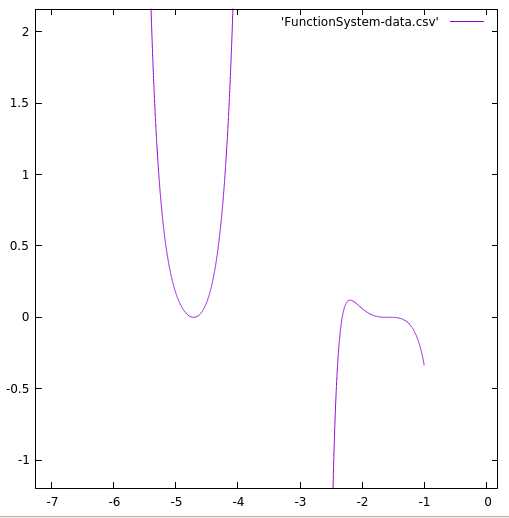
\includegraphics[width=300bp]{img/csv_tr.png}

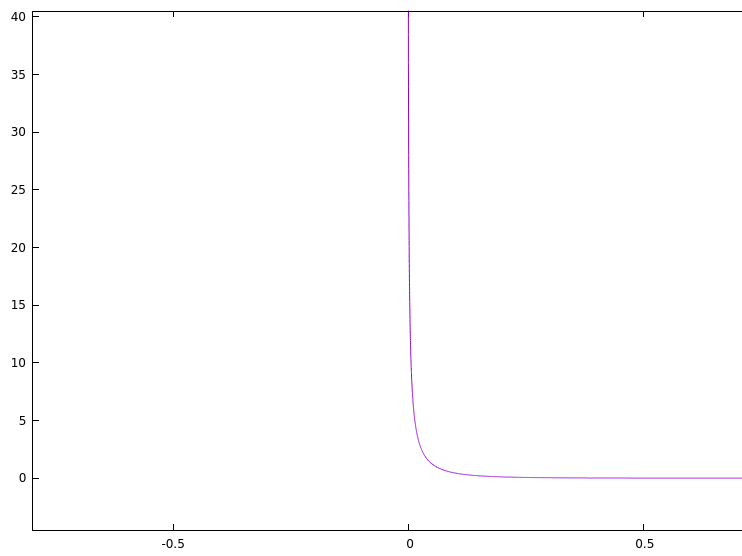
\includegraphics[width=300bp]{img/csv_ln.png}

\subsection{Выводы}
В ходе данной лабораторной работы были получены навыки разработки ПО с использованием интеграционного тестирования.

\end{document}
